\documentclass{article}
\usepackage{graphicx}
\usepackage{siunitx}
\graphicspath{ {images/} }
\title{First Pully Problem}
\author{Grant Curell}
\begin{document}
\maketitle{}
\section{Problem}
Here, the mass m isn’t moving, and you’re applying a force F to hold it stationary. Here’s the question: What force is the pulley’s support exerting, and in which direction, to keep the pulley where it is?

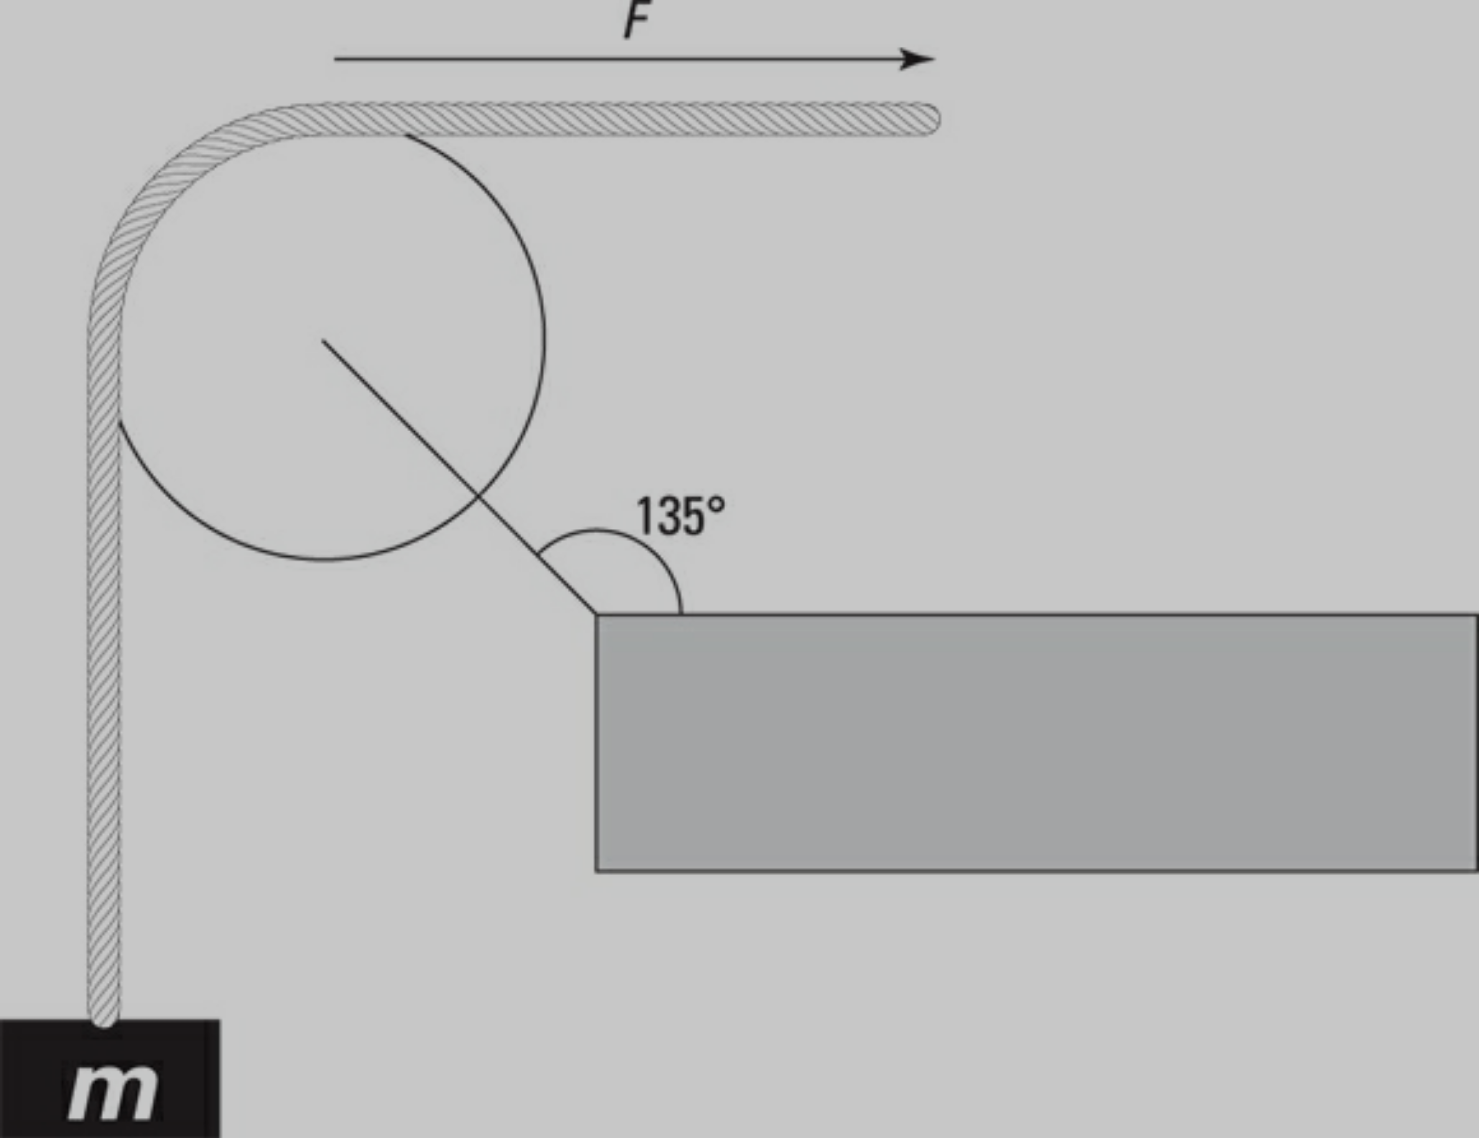
\includegraphics[width=\columnwidth]{image}
\\\\
Holzner, Steven. Physics I For Dummies (For Dummies (Math \& Science)) (p. 94). Wiley. Kindle Edition.
\\\\
\section{Solution}
\[ \sum F_y=F_{mass} \]
\[ \sum F_x=F_{manmeat pulling} \]
\[ \sum F_x=9.8m \]
\[ \sum F_y=-9.8m \]
Puesto que la acceleración del sistema es 0, sigue que las fuerzas tendrían
que igualar zero.
\[ \sum F_{support}=(-9.8m,9.8m) \]
\[ \sum F_{support}=\sqrt{(-9.8m)^2+(9.8m)^2} \]
The angle would be the same as the support so 135 degrees.
\end{document}
